%! Author = Luca Polese
%! Date = 31/03/2021

% Preamble
\documentclass[11pt]{article}

% Packages
\usepackage[utf8x]{inputenc}
\usepackage{amsmath}
\usepackage{tikz}
\usetikzlibrary{arrows,automata}

% Document
\begin{document}
    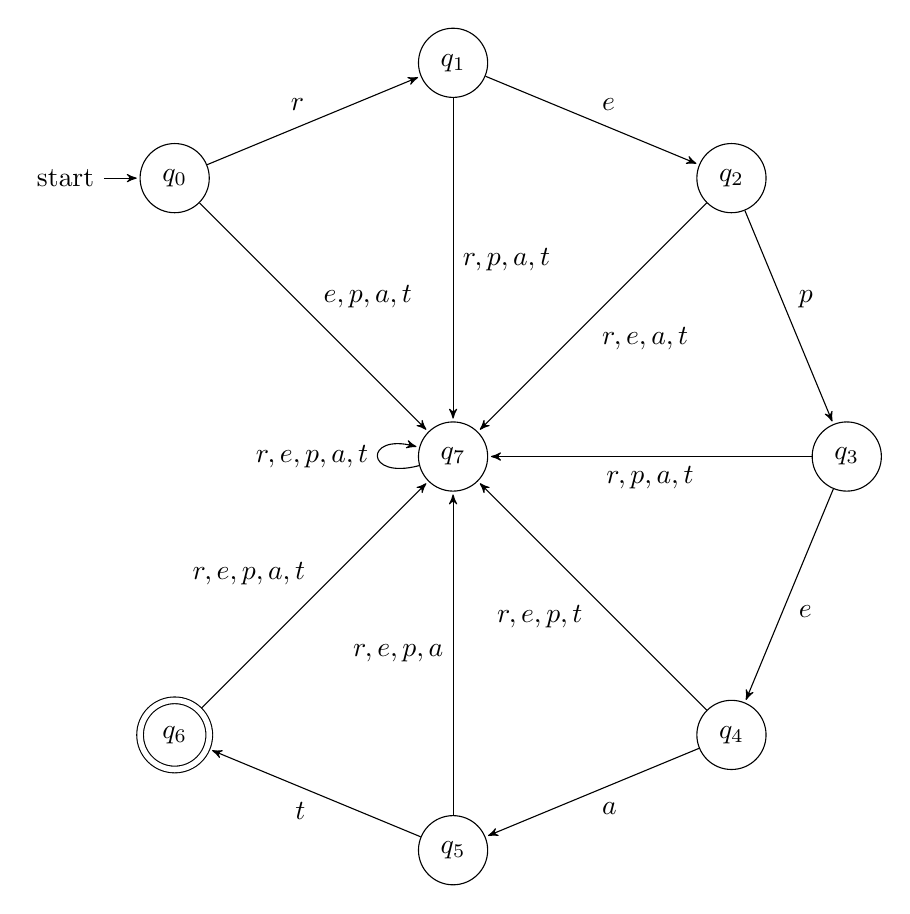
\begin{tikzpicture}[->,>=stealth',shorten >=1pt,auto,node distance=5cm,scale = 1,transform shape, accepting/.style={double distance=2pt, outer sep=0.75pt+\pgflinewidth} ]

        \node[state] (q_7) {$q_7$};
        \node[state,initial] (q_0) [above left of=q_7]{$q_0$};
        \node[state] (q_1) [above of=q_7] {$q_1$};
        \node[state] (q_2) [above right of=q_7] {$q_2$};
        \node[state] (q_3) [right of=q_7] {$q_3$};
        \node[state] (q_4) [below right of=q_7] {$q_4$};
        \node[state] (q_5) [below of=q_7] {$q_5$};
        \node[state,accepting] (q_6) [below left of=q_7] {$q_6$};


        \path (q_0) edge              node {$r$} (q_1)
        (q_1) edge              node {$e$} (q_2)
        (q_2) edge              node {$p$} (q_3)
        (q_3) edge              node {$e$} (q_4)
        (q_4) edge              node {$a$} (q_5)
        (q_5) edge              node {$t$} (q_6)
        (q_0) edge              node {$e,p,a,t$} (q_7)
        (q_1) edge              node {$r,p,a,t$} (q_7)
        (q_2) edge              node {$r,e,a,t$} (q_7)
        (q_3) edge              node {$r,p,a,t$} (q_7)
        (q_4) edge              node {$r,e,p,t$} (q_7)
        (q_5) edge              node {$r,e,p,a$} (q_7)
        (q_6) edge              node {$r,e,p,a,t$} (q_7)
        (q_7) edge  [loop left]            node {$r,e,p,a,t$} (q_7);

    \end{tikzpicture}
\end{document}